\documentclass{rspublic}   

%------------------------------------------------------------------------- 
% take the % away on next line to produce the final camera-ready version 
%\pagestyle{empty}

%\usepackage[utf8]{inputenc}
\usepackage{graphicx}
\usepackage{url}
\usepackage{float}
\usepackage{times}    
\usepackage{multirow}    
\usepackage{listings}   
\usepackage{times}     
\usepackage{paralist}    
\usepackage{wrapfig}    
\usepackage[small,it]{caption}
\usepackage{multirow}
\usepackage{ifpdf}   
\usepackage{subfigure} 

                    
%Bibliography                     
\usepackage{natbib}   

\usepackage{listings}
\usepackage{keyval}  
\usepackage{color}
\definecolor{listinggray}{gray}{0.95}
\definecolor{darkgray}{gray}{0.7}
\definecolor{commentgreen}{rgb}{0, 0.4, 0}
\definecolor{darkblue}{rgb}{0, 0, 0.4}
\definecolor{middleblue}{rgb}{0, 0, 0.7}
\definecolor{darkred}{rgb}{0.4, 0, 0}
\definecolor{brown}{rgb}{0.5, 0.5, 0}



\title[Efficient Replica-Exchange Simulations on
  Large-Scale Production Infrastructure]{Efficient Replica-Exchange Simulations on
  Large-Scale Production Infrastructure}

\author[Thota, Luckow, Jha]{
  Abhinav Thota$^{1,2}$, Andr\'e Luckow$^{1}$ and Shantenu Jha$^{1,2,3}$\\
  \small{\emph{$^{1}$Center for Computation \& Technology, Louisiana State University, Baton Rouge, LA 70803, USA}}\\
  \small{\emph{$^{2}$Department of Computer Science, Louisiana State
      University, Baton Rouge, LA 70803, USA}}\\
  \small{\emph{$^{3}$e-Science Institute, Edinburgh EH8 9AA, UK}}\\
}

%\date{}

\def\acknowledgementname{Acknowledgements}
\newenvironment{acknowledgement}%
{\section*{\acknowledgementname}%
\parindent=0pt%
}

\newif\ifdraft
\drafttrue
\ifdraft
\newcommand{\jhanote}[1]{ {\textcolor{red} { ***shantenu: #1 }}}
\newcommand{\alnote}[1]{ {\textcolor{blue} { ***andre: #1 }}}
\newcommand{\athotanote}[1]{ {\textcolor{green} { ***athota: #1 }}}
\else
\newcommand{\alnote}[1]{}
\newcommand{\athotanote}[1]{}
\newcommand{\jhanote}[1]{}
\fi

\newcommand{\I}[1]{\textit{#1}}
\newcommand{\B}[1]{\textbf{#1}}
\newcommand{\T}[1]{\texttt{#1}}

\newcommand{\glidein}[1]{Glide-In }  
\newcommand{\replicaagent}[1]{Replica-Agent }         
\newcommand{\remanager}[1]{RE-Manager }

\begin{document} 


\maketitle    

\begin{abstract}{Replica-Exchange, SAGA, Large-Scale, Production}  

  Developing applications that are able to orchestrate heterogeneous
  resources across distributed resources is a complex
  task. Inevitably, the design and development of an application is
  influenced and constrained by the programming systems and the
  infrastructure it is developed against. Breaking this coupling
  between the development and the underlying infrastructure, to enable
  applications to be flexible (across infrastructure), extensible (to
  new methods of communication and coordination) and scalable is an
  important design objective of both logically and physically
  distributed applications.  In this work, we focus on the
  Replica-Exchange (RE) Methods which represent a class of algorithms
  that involve a large number of loosely-coupled ensembles. RE
  simulations are used to understand physical phenomena Ð ranging from
  protein folding dynamics to binding affinity calculations.  In this
  work, we develop a flexible, extensible and scalable implementation
  of RE that can utilise a range of infrastructure concurrently
  \jhanote{(and autonomically/adaptively): Do we?}, that supports
  different coordination mechanisms (publish-subscribe \jhanote{do
    we?}, centralised notification), different replica pairing
  mechanisms (synchronous versus asynchronous) and thereby different
  variants of the RE algorithm. We implement and demonstrate how a
  flexible and robust implementation enables the efficient use of a
  broad range of infrastructure.

% Developing applications that are able to orchestrate heterogeneous
% resources across distributed resources is a complex task. Inevitably,
% the design and development of an application is influenced and
% constrained by the programming systems and the infrastructure it is
% developed against. Breaking this coupling between the development and
% the underlying infrastructure, to enable applications to be flexible
% (across infrastructure), extensible (to new methods of communication
% and coordination) and scalable is an important design objective of
% distributed applications both logically distributed and physically
% distributed.  In this work, we focus on the Replica-Exchange (RE)
% Methods which represent a class of algorithms that involve a large
% number of loosely-coupled ensembles. RE simulations are used to
% understand physical phenomena Ð ranging from protein folding dynamics
% to binding affinity calculations.  In this work, we develop a
% flexible, extensible and scalable implementation of RE that can
% utilise a range of infrastructure concurrently (and
% autonomically/adaptively), that supports different coordination
% mechanisms (publish/subscribe, centralized notification), different
% replica pairing mechanisms (synchronous versus asynchronous) and
% thereby different variants of the RE algorithm. We implement and
% demonstrate how a flexible and robust implementation enables the
% efficient use of a broad range of infrastructure.

\end{abstract}

\jhanote{please use \citep{} and not \cite{}}

\section{Introduction}
Developing applications that are able to orchestrate heterogeneous
resources across distributed resources is a complex task.  Inevitably,
the design and development of an application is influenced and
constrained by the programming systems and the infrastructure it is
developed against. Breaking this coupling between the development and
the underlying infrastructure, to enable applications to be flexible
(across infrastructure), extensible (to new methods of communication
and coordination) and scalable is an important design objective of
distributed applications -- both logically distributed and physically
distributed.

In this work, we focus on the Replica-Exchange
(RE)~\citep{hansmann,Sugita:1999rm} methods -- which represent a class
of algorithms that involve a large number of loosely-coupled
ensembles.  RE simulations are used to understand physical phenomena
-- ranging from protein folding dynamics to binding affinity
calculations. Most RE implementations are either infrastructure
specific (Woods et al. 2005) or, if using multiple distributed
resources, they require prior co-scheduling (Manos et
al. 2008). ~\citep{Luckow:2008fp} takes it to the next level and is an
example of adaptive RE simulations on production-level grid resources,
while ~\citep{parashar_arepex} is an example of \emph{asynchronous} RE
simulations, which is based on
CometG~\citep{Li:2005:CSC:1090948.1091381}, a decentralised
computational infrastructure for Desktop Grid environments.

We develop a flexible, extensible and scalable implementation of RE
that can utilize a range of infrastructure concurrently that supports
different coordination mechanisms (publish-subscribe, centralised
notification), different replica pairing mechanisms (synchronous
versus asynchronous) and thereby different variants of the RE
algorithm.  Application formulations that are scalable while being
flexible and extensible are better suited to using the diverse range
of traditional and hybrid infrastructure (e.g., Grid-Cloud and
heterogeneous resources).  

Along with application formulations that facilitate the flexible
utilisation of a range of infrastructure, it is imperative to have the
correct run-time abstractions that support flexible deployment of
these applications.  Consequently, we utilize a flexible pilot-job
implementation (SAGA BigJob) to support the execution of our
formulations.  We implement and demonstrate how a flexible and robust
implementation enables the efficient use of a broad range of
infrastructure. We compare and analyze the performance of the
different RE models (synchronous and asynchronous) when we scale-up to
256 replicas and scale-out to 4 machines. We present results using
which the reader can understand which model of RE is most suited for a
particular set of resources (distributed, local etc.,)

The rest of the paper is organized as follows. Section II sketches out
the different RE algorithms that we investigate. Section III outlines
the architecture of the SAGA BigJob and how it supports the dynamic
execution of multiple replicas (ensembles). In Section IV, we present
the implementation details of the RE algorithms and understand
the primary determinants of performance; we also present
an approximate mathematical model for the different algorithms.
% We also present
% different implementations of the asynchronous RE algorithm. 
In Section V, we describe the experiments performed with a view to
understanding the performance when scaling-up (on a single machine) as
the number of replicas increases. Section V also investigates the
scaling-out characteristics, namely performance as the number of
replicas are increased while the (distributed) resources employed
increases. %  while keeping the number of replicas on local and
% distributed resources. 
\jhanote{Currently we have only Section 6 and no 7}. In Section VI, we
present the results and analysis.  Section VII concludes the paper and
discusses future work.

% \alnote{Should we add a section with some scientific background: HIV,
%   Hepatitis...?}  \jhanote{given the tightness of space, I think we
%   should try to avoid it. OK?}

\section{Replica-Exchange Algorithms}
\label{sec:repex-approach}

% \jhanote{Abhinav: I still note the inconsistent and variable use of
%   algorithms, methods(?) and cases/approaches. I think we should refer
%   to Replica-Exchange as a ``class of algorithms'' or ``algorithm'',
%   and different implementations -- sync versus async} 

\athotanote{RE class of algorithms - synchronous and asynchronous
  models within RE class of algorithms; later sync, centralized-async,
  decent-async implementation. right? or - RE class of algorithms -
  synchronous and asynchronous implementation of RE class of
  algorithms; later sync, centralized-async, decent-async
  implementations. please suggest.}  \jhanote{I would say (i) RE Class
  of Algorithms, (ii) Sync/Async algorithms too, and then centralized
  or decentralized implementations of these sync versus async RE
  algorithm}
  
The RE class of algorithms involve the concurrent execution of
\emph{replicas} - which are defined as instances of essentially
similar simulations but with minor differences, such as the defining
temperature of the replica. These replicas are loosely coupled, in
that there is an infrequent exchange between pairs of % \jhanote{do we
%   want to say paired?} \athotanote{fixed}
replicas. In addition to the
frequency of communication between the replicas being small (relative
to within a single replica), the amount of information/data exchanged
between replicas is small (relative to the operating data-set
size). In the next subsection we develop a mathematical model which
aims to introduce the different components that make up the total
runtime of a RE experiment.

%\subsection{Mathematical Model}
%\alnote{I think we should discuss the mathematical model before going
  %into the specifics of sync/async RE.}

%Here we first provide a basic mathematical model for different RE
%models which explains the terms involved. In this section, we aim to
%develop an equation for total time to run any RE simulation. If $t$ is
%the average time between successful exchanges, and $p$ is the
%probability of a successful exchange,
%\begin{eqnarray}
%t=  {1 \over p} \times {[T_{MD} + T_{X} + T_{W}]} 
%\label{eq:timebtw}
%\end{eqnarray}

%where $T_{X}$ is the time to carry-out a pairwise exchange, which is
%comprised of (i) finding a partner, (ii) exchanging states including
%file transfer, (iii) book-keeping, and (iv) (re)starting the replica;
%$T_{W}$ is the time spent waiting for all replicas to complete running.


%Therefore, ${T_{X}} = {T_F + T_{ex} + T_{coord}}$ 

%and for ${T_{X}}^{async}, T_W = 0$

%The time ($T$) for N$_{X}$ exchanges is therefore $N_{X} \times t$

%If there are $\eta$ independent exchange events occurring
%concurrently, then the time $T$ for N$_x$ exchanges is $T \over \eta$.

\alnote{We should give a number for $\eta$ for sync
  RE}\athotanote{wouldn't that be implementation dependent?}
\alnote{What is the value of $\eta$ for async RE?} \athotanote{as
  mentioned earlier, i the value depends on the implementation;
  centralised=1, decentralised= $N_R\over2$} \athotanote{do we need
  the equation here again?}  \athotanote{I think
  $\eta_{sync,async-cent}$ should be 1 as only one exchange is done at
  a time(single master process) and $\eta_{async-decent}$ should be
  $N_R \over 2$, as each pair is involved in negotiating an
  exchange. since this depends on implementation, i am not including
  the $\eta$ values here.}

\subsection{Mathematical Model}
% \athotanote{i am not able to fit the sync, cent, decent
%   implementations into the math model. the problem is: $t$. in theory
%   $t$ may be possible, but if you look at the implementation, there
%   isn't a corresponding value. the exchanges don't happen in a way
%   where you could define $t$ in the way we define it in the original
%   math model. $T_{MD}$ of a single replica can't be considered for $t$
%   because replicas run in parallel, we don't have a distinct $T_{MD}$
%   for every $t$. }

Let us begin by considering an ideal scenario where there is no overhead involved in running an RE experiment. Then, the total time to complete an experiment would be equal to the concurrent runtime of the ensemble of replicas. In an RE experiment, the probability of a successful exchange is not 1. The decision to make the exchange or not is made using the Metropolis scheme (~\citep). In case of an unsuccessful exchange, the replicas are restarted without exchanging the configuration. Let the probability of a successful exchange be $p$. If the ensemble contains $N_R$ replicas, the total number of pairwise exchanges is $N_X$ and the runtime of a replica to complete a defined number of time steps is $T_{MD}$, then the total time to complete the RE experiment, $T$ would be: ${1 \over p} \times T_{MD} \times {N_X \over {N_R \over 2}}$. %At this point, let us define the term \emph{generation} as one concurrent run of the ensemble of replicas. Thus, after each generation, exchangs are made and the replicas restarted. 
But it is not actually possible to implement an RE experiment without overhead. A more practical equation for total time would look like this.
\alnote{Why is the second $N_X$ not divided by $\eta$}
\begin{eqnarray}
T = {1\over p} \times [(T_{MD} \times  {N_X \over {N_R \over 2}}) + (T_{EX} + T_{W}) \times N_X]
\label{eq:totaltime}
\end{eqnarray}

Where $T_{EX}$ is the time to make a pairwise exchange and would
include components like time to find a partner ($T_F$), time to
exchange files or to write and transfer files ($T_{ex}$) and
book-keeping ($T_{coord}$). $T_W$ is the time spent by a replica
waiting for other replicas to become available ($T_W$), the time spent
waiting till it is restarted after each exchange ($T_r$) and any other
miscellaneous costs. Thus $T_{EX} = T_{F} + T_{ex}+T_{coord}$ and
$T_w=T_w+T_r$.  \alnote{Using ex and EX as subscripts is very
  confusing!} \jhanote{Why not use T$_X$ in lieu of $T_{EX}$? }

Equation \ref{eq:totaltime} gives the total time to complete an RE
experiment. The next equation aims to calculate the time to complete
particular number of exchanges ($N_z$), where $0 \geq N_z \geq N_X$.

\begin{eqnarray}
T_z = {1\over p} \times [(T_{MD} \times  \lceil{N_z \over {N_R \over 2}}\rceil) + (T_{EX} + T_{W}) \times N_z]
\label{eq:parttime}
\end{eqnarray}

Here $\lceil$ $\rceil$ denotes the ceiling function. The reason we put the term ${N_z \over {N_R \over 2}}$ under a ceiling function is because the ensemble of replicas run concurrently and for each concurrent run, $N_R \over 2$ exchanges are possible. Therefore, only the coordination and waiting costs effect the total time. 

Also, if there are $\eta$ independent exchange events occurring
concurrently, then the time $T$ to complete the RE experiment where N$_X$ is the total number of exchanges is:

\begin{eqnarray}
T = {1\over p} \times [(T_{MD} \times  {N_X \over {N_R \over 2}}) + {(T_{EX} + T_{W}) \over \eta} \times N_X]
\label{eq:totaltime2}
\end{eqnarray}

\athotanote{please suggest alternative terms if you find anything confusing}

%It should be noted that only the coordination and waiting costs are divided by $\eta$. The ensemble of replicas are already running concurrently and 


% The RE algorithm involves the concurrent execution of multiple similar
% simulations, the \emph{replicas}.  There is a loose-coupling between
% the replicas in form of periodic exchange attempts between paired
% replicas. The traditional approach to RE is the synchronous model,
% which works well in an ideal scenario with a well defined model of
% resource availability. But with heterogenous systems and fluctuating
% resource availability, the asynchronous RE model could be more
% effectively used to conduct simulations. 
% >>>>>>> .r3441


%Previously, we demonstrated the usage of the SAGA Pilot-Job
%framework~\citep{saga_bigjob_condor_cloud} -- called the BigJob, to run
%RE simulations across multiple, heterogeneous distributed Grid and
%Cloud infrastructures~\citep{Luckow:2008fp}.
%\alnote{maybe we should also intro SAGA at some point} \jhanote{Yes} The Simple API for Grid Applications (SAGA)~\citep{saga_gfd90} is an API standardization effort within the Open Grid Forum (OGF)~\citep{ogf_web}, an international standards development body concerned primarily with standards for distributed computing. The various tasks that are carried out using the SAGA APIs include file staging, job spawning and the conduction of the exchange attempts.
%Further, we introduced several adaptivity modes, e.\,g.\ adaptive
%sampling that are able to react to dynamic changes in resource
%availabilities.

%\alnote{Not sure how many technical we need to provide...}  

%Traditionally, depending
%on the number of processes \texttt{N}, the manager creates \texttt{N/2} pairs
%of replicas.  Before launching a job, the manager ensures that all
%required input files are transferred to the respective resource. For
%this purpose, the SAGA File API and the GridFTP adaptor are used. The
%replica jobs are then submitted to the resource using the SAGA CPR
%API and the MIGOL/GRAM middleware.

%\jhanote{Mention that these are SAGA-based implementations. Something  else would be implemented differently}
%\alnote{Proposed structure: a) math. model b) sync c) async. We should give the reader some orientation in this section.}

\subsection{Synchronous Replica Exchange}

%\alnote{Are we already introducing cases in this sec?} \athotanote{nope, i don't think so!}
  In the synchronous (traditional)
model of the RE algorithm, depending upon on the number of replicas ${N_R}$, 
${N_R \over 2}$ pairs of replicas are created. When \emph{all} the replicas in the ensemble reach a
pre-determined state (e.g. the MD simulation completes a pre-determined
number of steps), % a decision as to whether to exchange temperatures
%between previously
an exchange of temperatures between the paired replicas is attempted
using the Metropolis scheme. %  The ensembles of replicas executes
% concurrently, and the subsequent pairwise exchange attempt are
% referred to as generation. No two replicas can belong to different
% generations. 
If the exchange attempt is successful, parameters such as the
temperature are swapped. Both jobs are then
restarted~\citep{Luckow:2008fp}.

%As mentioned in the equation (~\ref{eq:totaltime}), if $T$ is the total time to complete RE experiment and $p$ the probability of a successful pairwise exchange, then:

%$T = {1\over p} \times [T_{MD}+ [T_{X} + T_{W}] \times N_X]$

%It should be noted that we are discussing the average values of each of the term in the equation above.
%If there are $\eta$ independent exchange events occurring concurrently, then the time $T$ for 
%N$_x$ exchanges is $T \over \eta$.

% \jhanote{let us be consistent. Is the entire RE process/workflow a
%   simulation or is an individual replica/task a simulation? I prefer
%   the latter, in which case the T$_C$ is not of a simulation but that
%   of a RE run/work/process?} \athotanote{i am calling the whole RE
%   process/worklow as an RE experiment}

In equation \ref{eq:totaltime2}, we introduced the various components
that make up the total time to complete an RE experiment. Only the
coordination and waiting costs would differ with different models of
the RE algorithm. That would be the terms $T_{EX}$ and $T_W$. In a
synchronous RE experiment, since all the replicas complete running
before the exchanges are made, $T_F = 0$. And $T_W$ would include the
time waiting for all the replicas in an ensemble running concurrently
to complete running, the time spent waiting before the replicas are
restarted after each exchange and any other miscellaneous costs.

 % 1 para limitation on traditional replica exchange

A major limitation of this model is that the replicas are paired in
fixed groups and thus exchanges take place between pre-determined
pairs of replicas.  This limits the number of possible exchange
partners that are available for a given replica, and thus also
inhibits exchanges between replicas with non-nearest temperatures, and
ultimately negates the possibility of crosswalks. (A crosswalk is said
to occur when a replica originally with a low temperature reaches the
upper temperature range and then returns to the lower temperature
range.)  Rigid replica-pairing works well in a homogeneous
environment, but with heterogeneous systems, where the resource
availability and performance fluctuates, the need for synchronisation
leads to slow-down \& inefficiencies.

 
\subsection{Asynchronous Replica Exchange}
%- Introduce asynchronous Replica Exchange --  1 para on case II and case III (algorithmically)

%To overcome these limitations

We take the asynchronous RE algorithm proposed by
~\citep{parashar_arepex}, ~\citep{??} \jhanote{Also please cite the
  JCC paper of Gallichio, Levy and Parashar. See references/ directory
  please} and implement it on distributed grid resources. By
asynchronous, we mean that a replica does not have to wait for all the
replicas to finish running. An exchange occurs whenever a pair of
replicas are available, and where a replica can perform exchanges
asynchronously with any other replica in the ensemble.
% \jhanote{Is the algorithm similar or identical? If it is not
%   identical, how is it different, or is it just the case that the
%   implementation is different?} \athotanote{is it ok now? i think we
%   are taking the async algorithm as is and implementing it on
%   production infrastructure. ?}

Let us look at how the coordination and waiting costs introduced in
equation \ref{eq:totaltime2} behave. That would be the terms $T_{EX}$
and $T_W$. In an asynchronous RE experiment, since each replica on
completing a run has to find a partner, $T_F \neq 0$. And $T_W$ would
only include the time spent waiting for the next replica to become
available, any time spent waiting before the replicas are restarted
after an exchange and any other miscellaneous costs.

%\alnote{This is too general.   We should drop the redundancy of explaining every component and rather analyze the differences.} \athotanote{you are right; i am adding a couple of lines here. does it help?} \jhanote{As currently written, $T_W$ has not been defined or ``different components'' discussed, i.e., this paragraph should come after the modelling section}

% But also, an asynchronous RE algorithm has the potential to perform
% better than the traditional RE: (i) when we scale-up the number of
% replicas and (ii) when we scale-out across many machines.
%\jhanote{There is no basis for this sentence at the moment. REMOVE}


\section{Replica-Exchange Framework}

The RE Framework we present is independent of the underlying infrastructure and provides the capability to implement a variety of RE algorithms. 
An important motivation for us to come up with an RE Framework is to present an infrastructure independent solution that makes it possible to implement a variety of RE algorithms, such as synchronous and asynchronous, that can dynamically utilise a range of infrastructures.
 It is also important to have a scheme
that does not depend on a static set of resources that are pre-defined
at the time of workload submission.  
% \jhanote{If we are talking about differences in the impelementation,
%   then that does not belong here. If we are talking about the
%   algorithm, then it belongs here} \athotanote{moved this from section 2 to here}
   We differ from the implementation described
in \citep{parashar_arepex} in some important ways.  The asynchronous
RE model we developed runs on production level grids such as the
Teragrid and LONI~\citep{LONI_web}, unlike specialized
infrastructures. % \jhanote{Careful. Comet is only a
% coordination infrastructure which can be overlayed over production
% CI} \athotanote{removed cometg. is it accurate now - specialized
% infrastructure?}
Also, we run the replicas as MPI jobs. In following subsections we introduce the different components in the RE Framework. 
  
  
  %\jhanote{have not defined  asynchronous implementation yet!}  \alnote{Also, I think we should  focus more on the algorithm than on the deployment  aspects}\jhanote{I echo Luckow's remark. And my remarks reflect that  too}

\subsection{SAGA BigJob - A Pilot-job Framework}
\label{sec:BigJob}

The Simple API for Grid Applications (SAGA)(~\citep{saga_gfd90}) is an
API that provides the basic functionality required to build
distributed applications, tools and frameworks so as to be independent
of the details of the underlying infrastructure. SAGA is an API
standardization effort within the Open Grid Forum
(OGF)~\citep{ogf_web}, an international standards development body
concerned primarily with standards for distributed computing. The
various tasks that are carried out using the SAGA APIs include file
staging, job spawning and the conduction of the exchange attempts.


%%%%% FIGURE %%%%%
\begin{figure}[t]
      \centering
          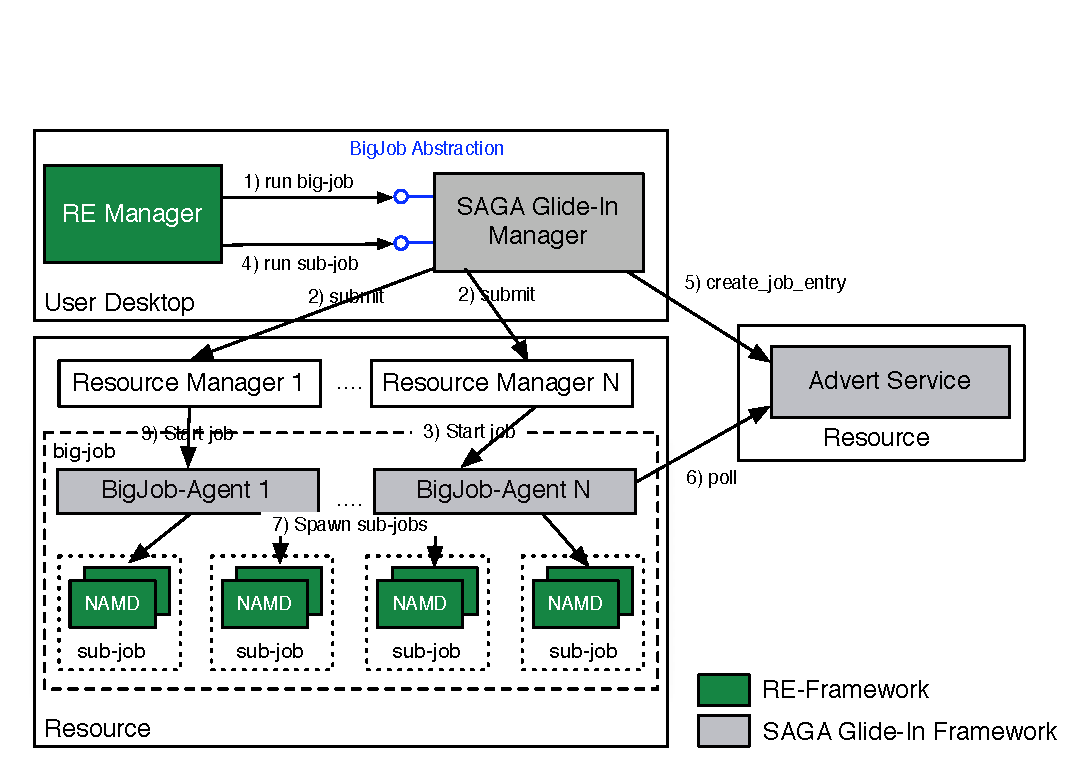
\includegraphics[width=0.82\textwidth]{../figures/Bigjob_arch.pdf}
          \caption{\footnotesize SAGA/BigJob Architecture
              }
      \label{fig:bigjob}
\end{figure}

Previously, we demonstrated the usage of the SAGA Pilot-Job
framework~\citep{saga_bigjob_condor_cloud} -- called the BigJob, to
run RE simulations across multiple, heterogeneous, distributed grid
and cloud infrastructure~\citep{Luckow:2008fp}. Here we use the BigJob
framework to efficiently request and manage computational resources
for multiple replicas.  Figure ~\ref{fig:bigjob} shows the
architecture of SAGA BigJob.  It consists of three components: (i) the
SAGA-BigJob Manager, (ii) the BigJob Agent and (iii) the advert
service. The SAGA-BigJob manager submits the BigJobs to the resource
manager and the sub-job descriptions to the \emph{advert server}. The
advert server can be on any machine and is a central key/value store
which is used for communication between the SAGA-BigJob Manager and
the BigJob agent. There is a separate BigJob agent for each
BigJob. Thus, every BigJob on every machine has a local BigJob
agent. Once the BigJobs become active, the BigJob agent retrieves the
job descriptions from the advert server, allocates the required number
of nodes and launches the sub-jobs on each resource. The BigJob agent
continuously monitors the running sub-jobs and updates the sub-job
states in the advert server. Once a sub-job finishes running, the
nodes are freed and marked as available. The BigJob agent periodically
polls the advert server for new jobs.

\subsection{Replica-Exchange Manager}\label{repexmanager} 

% \jhanote{Abhinav: This subsection should help the reader understand
%   the basic and common elements of the RE Framework -- job submission,
%   role of bigjob-agent, replica agent, replica-exchange manager etc
%   etc} \athotanote{job submission, bigjob agent are explained in 3a. RE Manager is explained below. replica agent is touched upon but a more detailed explanation in section 3b(ii)}
  
%   \jhanote{ABHINAV: DEFINE THE ROLE OF RE-MANAGER HERE.  Possibly BIGJOB
%   AGENT here if not in previous subsection.}  \athotanote{please check if it's ok now}
  
The RE Manager is an abstraction over the SAGA BigJob Manager. At the most, the RE Manager is the master process controlling all the aspects of the RE experiment and exchanges. And at the least, it is the SAGA BigJob Manager. The actual tasks that the RE Manager carries out depend on the type of the implementation. In an implementation where the RE Manager manages all the replicas and makes all the exchanges, the RE Manager does a lot of work (a centralized implementation). But in an implementation where there is a \emph{replica agent} for every replica, the RE Manager has the same functionality as the SAGA BigJob Manager (a decentralized implementation). A replica agent is a wrapper script launched in place of the replica. The replica agent typically manages the replica and makes the exchanges. It should be noted that synchronous and asynchronous RE are the different algorithms and the implementation of an same algorithm could be centralized and decentralized.

%Synchronous RE is implemented in a centralised fashion. Centralized implementation suits synchronous RE because there is a synchronization step at the beginning of each exchange step. But we implement asynchronous RE in both centralised and decentralised fashions. 

The actual tasks that the RE Manager carries out depending on the implementation are explained in the following sections. 
We explain how the synchronous and asynchronous (centralized) RE Manager works in the following section and in the section following that explain how the asynchronous (decentralized) RE Manager/replica agent combination works. We explain synchronous and asynchronous (centralized) RE Managers in the same section as they are both centralized implementations and have a lot of similarities. 

% The RE-Manager also creates directories, configuration files and stages them to the respective directories.  \alnote{We should focus on the RE part here. The BigJob  stuff move to subsec a). This should also remove the redundancy with  a)} 

\begin{figure}%
\centering
\subfigure[Central]{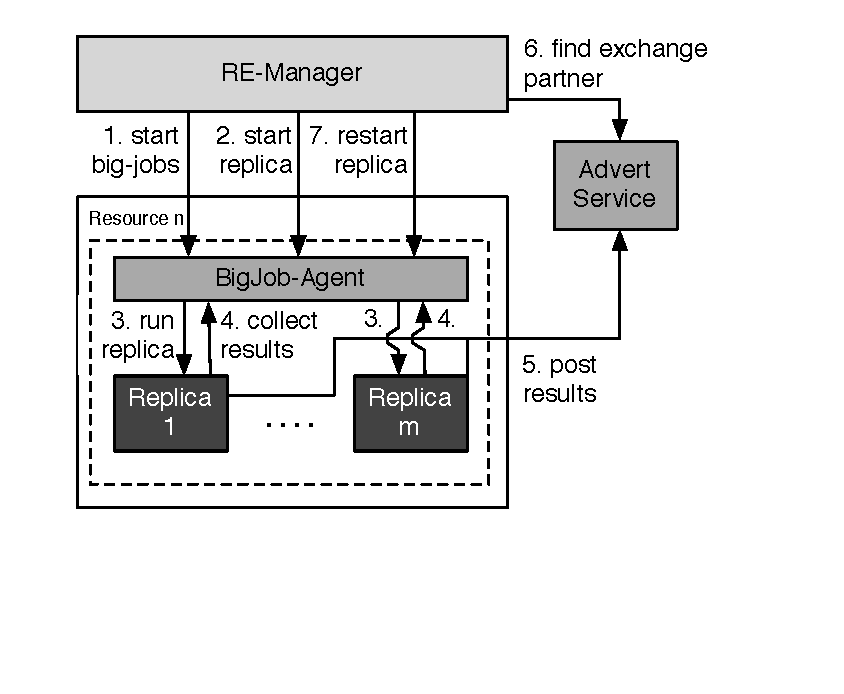
\includegraphics[width=0.47\textwidth]{../figures/central_AL.pdf}}\qquad
\subfigure[Decentral]{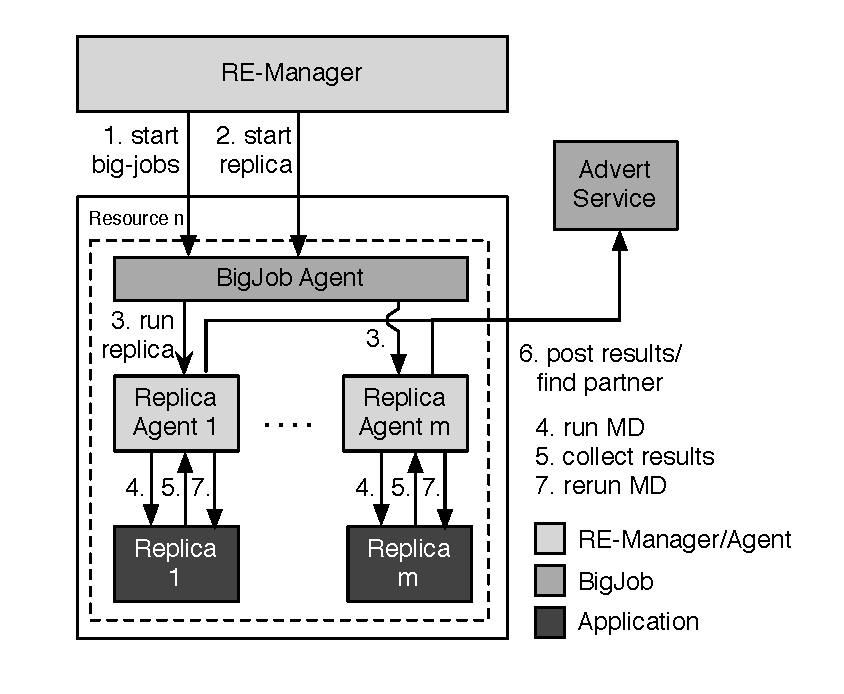
\includegraphics[width=0.47\textwidth]{../figures/decentral_AL.pdf}}\\
\caption{\textbf{Centralised vs. Decentralised Coordination:} Both
  central coordination style is used both by the synchronous RE (case
  I) and a version of the asynchronous RE (case II).  In the decentral
  style -- used by another version of the asynchronous RE (case III)--
  the master is only required for initially setting up all
  replicas. The later coordination is done peer-to-peer via the Advert
  Service.}
\label{fig:coordination}
\end{figure}

\subsubsection{Synchronous and Asynchronous (centralized) RE-Manager}

Here we first explain how the synchronous RE Manager works and then explain asynchronous (centralized) RE Manager. The control flow of the asynchronous (centralized) RE case is shown in
Figure~\ref{fig:coordination}a). But as synchronous RE is also a centralized implementation, we use it to describe both. %\jhanote{Abhinav, please check that  this is correct?}

Once the BigJobs are running and the replicas are running, the RE Manager constantly queries the SAGA BigJob Manager for the latest replica states. \alnote{The RE-Manager queries BigJob. We should hide
  the BJ impl details in this section.}  When the RE-Manager finds a
replica that has finished running, it collects the energy and
temperature of that replica by reading the output file. Once
\emph{all} the replicas have finished running, the RE-Manager makes
the exchanges. The exchange is done by exchanging the temperatures and
writing new configuration files. The new configuration files are staged to the appropriate location. The RE-Manager then submits the replicas for restarting.  \alnote{The RE-Manager spawns a new sub-job. BJ uses the
  advert service to dispatch this subjob. See comments above} The
BigJob agent finds the replicas and restarts them. The RE-Manager
counts the successful exchanges. This process is repeated until the
required number of exchanges are done.

The architecture of an asynchronous (centralized) RE-Manager is similar to that of synchronous RE Manager. 
Figure~\ref{fig:coordination}a) shows the control flow. The difference is that instead of waiting 
for \emph{all} replicas to finish running before making exchanges, whenever the 
asynchronous (centralized) RE-Manager finds a replica that 
has finished running, it tries to find a partner to make an exchange. In order to find a partner, the RE Manager goes over the list of all the replicas in the ensemble. If it finds a replica available it attempts the exchange. If a replica is not found available, the RE Manager queries the SAGA BigJob Manager for the latest replica states and updates its local list. It then loops over the list to find a replica that has finished running and a partner to exchange with that replica.
If successful, the replicas are submitted to be restarted. \alnote{see comment about BJ impl. detail above}. 
The RE-Manager counts the successful 
exchanges. This process is repeated till all the exchanges are made. 

\alnote{Not sure what we should do with the following paragraph}
\jhanote{Does not belong here} It should be noted that where as in the
synchronous RE, the exchanges are conducted when all replicas finish
running. And the replicas are restarted only after all the exchanges
are completed. But in an asynchronous (centralized) RE, the exchanges
are conducted whenever possible and the replicas are restarted.

\subsubsection{Asynchronous (decentralized) RE-Manager and the replica agent}

In the asynchronous (decentralized) implementation, the RE Manager's responsibility is greatly reduced and it only needs to keep count of the number of exchanges completed. When the required number of exchanges are done, the RE Manager ends the experiment. 

In order to conduct the exchanges in a decentralized fashion, replica-agents are launched in place of replicas. As mentioned earlier, the replica agent is just a wrapper script for the replica, which starts, makes exchanges and restarts the replica. Thus, after the replica-agents are launched, the RE Manager and the SAGA BigJob Manager don't have any responsibilities.  

\jhanote{ISNT THE NEXT PARAGRAPH ESSENTIALLY THE SAME AS THE PREVIOUS
  PARAGRAHGP? WHY DONT YOU REFER TO THE FIGURE AND THE BASIC StePS
  OUTLINED IN THE FIGURE?}
  
\begin{figure}[t]
      \centering
          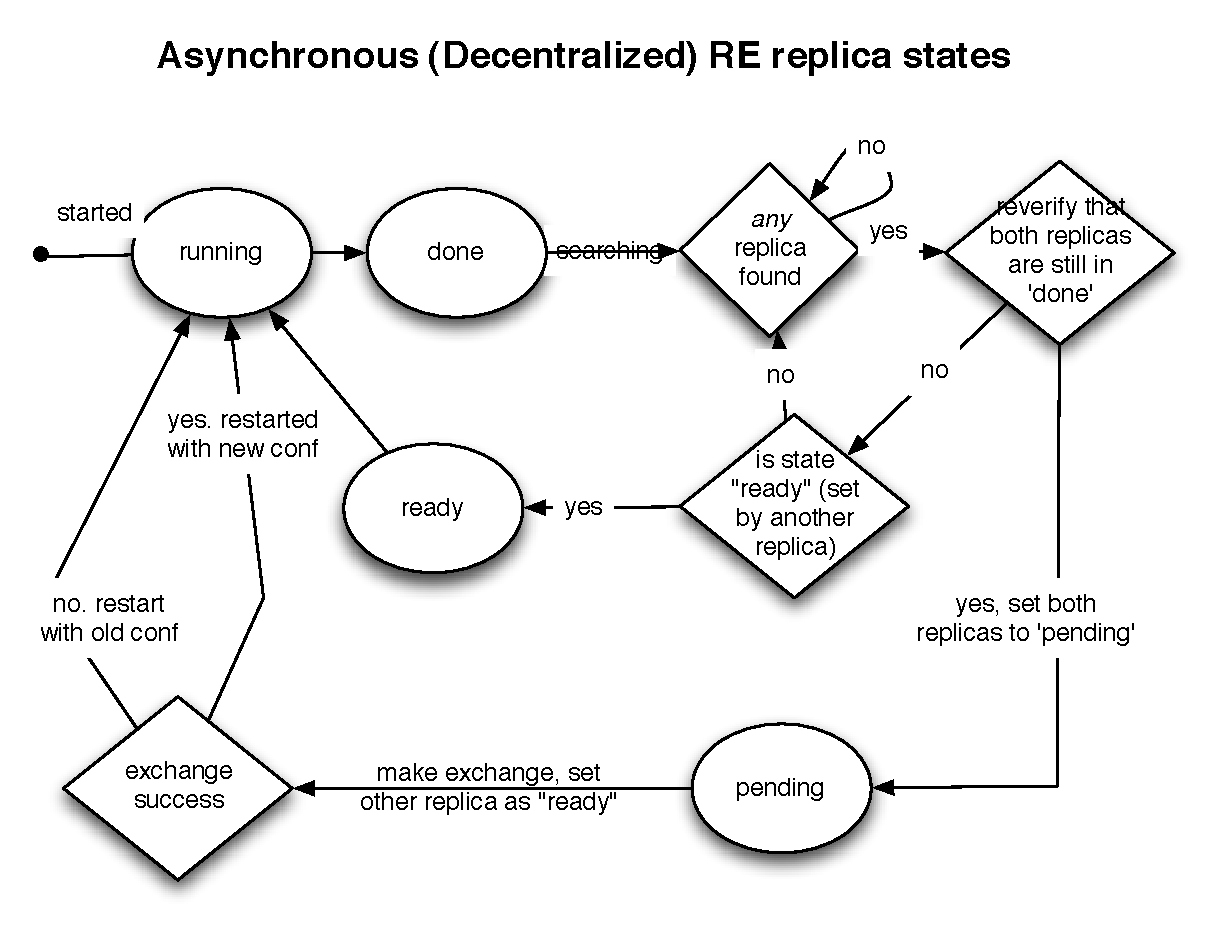
\includegraphics[width=0.82\textwidth]{../figures/decent_state.pdf}
          \caption{\footnotesize Asynchronous (decentralized) RE replica state diagram
              } \alnote{This chart is not correct yet. There can't be state changes on conditional fields}
      \label{fig:state}
\end{figure}


Figure~\ref{fig:coordination}b shows the asynchronous (decentralized) RE
control-flow. Figure \ref{fig:state} shows the replica state diagram. The replica agent upon launch, runs the replica. The nodefile is passed to the replica agent as an argument at startup. The replica agent constantly monitors the replica and when the replica finishes its run, it updates the advert server with
the current state of the replica. It also reads the temperature and
energy from the output files and posts the values to the advert
server. It then goes through the list of replicas in the ensemble in a random order and tries to find an
exchange partner. The search for an exchange partner is conducted in a random manner so as to avoid having all the replicas starting at the first replica, which causes contention and failed exchanges. If it finds another replica available, it
re-verifies the states of both itself and the other replica and if it
finds both still available, marks their states as "Pending". Let the replica initiating the exchange be $R_a$ and the other replica be $R_b$.
The replica $R_a$ which initiates the exchange is the replica in-charge of the exchange. $R_a$
then exchanges their temperature values on the advert server.  \alnote{We
  should detail the exchange protocol. How do we ensure that the
  exchange is atomic? figure?}  It then modifies its configuration
files locally, sets its state as running and runs the replica. On the
other hand, the $R_b$'s state is set as "Ready" by $R_a$ and that
makes the $R_b$'s replica agent to retrieve its own
temperature (modified by the $R_a$) from the advert server, modify its configuration file
locally and run the replica. \alnote{Why does it need to modify its
  own config if it uses its own temperature?} \athotanote{fixed} This removes the need to stage the configuration files to
different machines. This is possible because there is a replica agent
for each replica locally. Where as earlier, the RE-Manager and the
replica might be located on different machines. 
  If the state of any of the replicas negotiating the exchange changes at the time of re-verifying the replica pair's states, that would mean that one or both of the replicas' is now in the process of making an exchange with a different replica. In that case one or both of the replica agents will wait till their state is set as "Ready" and start their next run. If one of the replicas is still available, it tries to find a new partner for exchange.  \alnote{How often is the process repeated until the replica
  is started with the old temperature?} \athotanote{fixed}The replica agent that
initiated the exchange increments the exchange count by one.
If an exchange fails due to contention, the replica agent tries to find a new partner. If an exchange is deemed unsuccessful after comparison of energies or temperatures, the replicas are restarted with their old configurations. 

\jhanote{Do we have a pending state? Accoridng to Abhinav there is
  only a two-state model -- run and done?!} \athotanote{should i keep the state diagram? do you suggest any corrections to the state diagram? i also think that instead of having the current control flows, we should have figures showing how the exchanges are made or instead hae state diagrams. the control flows right now show a lot of stuff already shown in the bigjob architecture figure. }
  

\section{Implementation of Synchronous and Asynchronous RE}

% \jhanote{This section should help the reader understand the control
%   flow - which is YOUR IMPLEMENTATION of the RE algorithm. Need to
%   make reference to Figures 2a and 2b} \athotanote{i think we are doing this in section 3?}\jhanote{Yes}

% \alnote{General remark: What do you guys think of summarizing the data into 
% a table? This way the reader can track the numbers at one central place.}
% \jhanote{YES. I have suggested the same too}

We present the implementation costs of the synchronous RE and the
asynchronous (centralized and decentralized) RE implementations here.
% \jhanote{Explain centralized and decentralized} \alnote{The question
%   is: where do we explain it? There are already a lot of details in
%   sec III}\jhanote{Yes. Old remark. Will be removed}


\begin{table}
    \centering
	\begin{tabular}{|l|c|c|c|}
	\hline
	                        &sync. RE &async central. RE &async decent. RE\\
	\hline
	$T_{MD\_init}$  &23\,sec &23\,sec &23\,sec\\
	\hline
	$T_{MD\_run}$   &68\,sec &68\,sec &68\,sec\\
	\hline
	$T_{F}$           &0\,sec &&\\
	\hline
	$T_{W}$           &&&\\
	\hline
	$T_{EX}$          &&&\\
	\hline
	$T_{COORD}$       &&&\\
	\hline
	\end{tabular}
	\caption{Replica-Exchange Performance}
	\label{table:repex_perf}
\end{table}


In order to be able to discuss the various costs involved, 
which will depend on the configuration for the RE experiment, 
the configuration we set for synchronous and asynchronous RE is explained below.

Nanoscale molecular dynamics (NAMD)
(Phillips et al.  2005), a highly scalable, parallel MD code, is used
to carry out the MD simulation corresponding to each replica run. It
is important to mention that any other MD or Monte Carlo code could be
used just as simply and effectively. The total number of
replicas ($N_R$) in the ensemble are 32 and the total number of
pairwise exchanges ($N_X$) is 128. As the ensemble of replicas are run concurrently, 16 pairwise exchanges are possible after each concurrent run. Thus, each replica on average is restarted 7 times.
Our experiments are performed on
LONI and Teragrid shared resource \emph{QueenBee}. Each replica is
configured to run 500 time-steps and is allocated 16 processors. It
should be noted that we are talking about the average values whenever
we mention quantities. Each replica takes 91 seconds to complete the
500 time-steps from a fresh start and 68 seconds every time it is
restarted. Thus, if each replica is restarted 7 times, the average
time to complete 500 time-steps ($T_{MD}$) is ${(91+68\times 7) \over8} = 71$ seconds. 
\alnote{The 71\,sec average won't hold for larger $N_{x}$}
It should be noted that the replicas take longer (91 seconds) 
to complete their 500 time-steps from a fresh start. But when 
they are restarted, they finish the run slightly faster (68 seconds).   
And the total time the ensemble of replicas spend running is $71 \times 8 = 568$ seconds. 
  
Also, we are primarily
interested in learning the scale-up and scale-out properties of
synchronous and asynchronous RE and hence are not concerned by the
queue wait time. Therefore, we only start measuring when the BigJob agent starts running the replicas. Because, almost every time, the RE Manager completes submitting the replicas before the BigJob becomes active.

\subsection{Synchronous RE}
The replicas are run by the BigJob agent after the BigJob becomes active. The average 
time the Bigjob agent takes to start one replica is 0.3 seconds.  
\alnote{Is this the time agent only? Or does it include the submission time on the master?} 
\athotanote{fixed in last lines of the previous section. the time the master takes 
to submit the replicas is being included in $T_EX$. The time spent at BigJob agent 
is included in $T_W$. }  \alnote{Don't see any reference to $T_{EX}$ in last section. Later you
refer to the resubmission time as $T_{coord}$. Also, I don't see this component in the 
$T_W$ formula below. The reader will not know what to do with the 0.6 sec!}
For a pair of replicas, it is 0.6 seconds.

The BigJob agent takes 0.92 seconds to process a replica that completes running. 
That is the time it takes to update the state and
mark the nodes as free. For a pair of replicas it is 1.84 seconds. But since the 
whole ensemble of replicas need to complete running, it is sufficient to 
consider the longer of the time to start and the time to mark the end of a replica run.
The RE-Manager periodically queries
the advert server for the latest replica states and marks the replicas
which finish running as done and retrieves the current energies and
temperatures by reading the output files. This takes 0.4 seconds per
replica and for a pair of replicas, it is 0.8 seconds. 
Thus, the cost of making a pair of replicas available to the RE Manager 
for exchanges is $T_W$ = 1.84+0.8=2.64 seconds. 
\alnote{What is the component that is actually spent waiting for the other replicas
to complete. The times you mention above are times for actually doing something, but
not waiting times!}

Since all the replicas finish running before
the exchanges are started, the RE manager won't spend any time
searching for partners and $T_F$ is 0 seconds. $T_{ex}$ includes
updating configuration files and transferring the them to their
respective directories, in this case, locally. It takes 0.2 seconds to
write and copy a file locally. $T_{ex} = 0.2 \times 2=0.4$
seconds. $T_{coord}$ is the time required by the RE-Manager to resubmit 
the pair of replicas using BigJob. In average $T_{coord}$ amounts to 
$0.11\,sec \times 2 = 0.22\,sec$. Therefore, $T_{ex}$ is $0+0.4+0.22=0.62$ seconds.
\alnote{We need to decide whether we use capital letters or not: $T_{ex}$ vs. $T_{EX}$}
Substituting the above values in equation~\ref{eq:totaltime}, we get
\begin{eqnarray}
T=  {1 \over p} \times {[ {(71\times {128\over 16}})+ (0.62 + 2.64)\times 128]} = {1 \over p} \times (990)
\label{eq:sync}
\end{eqnarray}
%\alnote{$T_{MD}$ should be also x Nx?}


\subsection{Asynchronous (centralized) RE}
\alnote{please don't just copy paste. Only focus on the differences}

%As before, the average time the BigJob agent takes to
%start one replica is 0.3 seconds. For 32 replicas, it is 9.6
%seconds. Thus, the BigJob agent finishes starting the last replica before the a replica completes its run. 

%The BigJob agent
%would be ready to restart the replicas by the time the RE-Manager
%submits to the advert server. %\alnote{Not consistent with a) Where is the 71s number?}

As mentioned earlier, the BigJob agent takes 0.92 seconds to find that
a replica is done, update the state and free the
nodes. But in this implementation, we also make the BigJob agent also 
retrieve the energy and temperature from the output files, which 
adds 0.2 seconds per replica. Therefore it takes 1.12*32=35.84 seconds 
for 32 replicas. But even as a pair of replicas are marked as done 
by the BigJob agent, the
RE-Manager concurrently makes exchanges between other pairs of
replicas - and that pair of replicas would wait approximately 32 seconds before the BigJob agent is able to them. It should be noted that the timelines of the RE-Manager and the BigJob agent run partly concurrent and partly serial to each other.  As the simulation progresses, as pairs of replicas are restarted instead of
all the replicas starting and ending together, groups or pairs of
replicas start and end at the same time. The pairs
of replicas belonging to the first few exchanges might have waited the
32 seconds at the BigJob agent, but we observed that groups of
replicas belonging to the later exchanges wait for only half that
amount of time. This is because the BigJob agent would move between ending and starting replicas more frequently. That is 32/2 = 16. For a pair of replicas, $T_W$ is 16/16 =1 second is the waiting cost.

The time the RE Manager takes to find a partner ($T_F$)
depends on $N_R$ and also on the number of replicas the RE-Manager has
to sift through to finds an available replica. On average, RE-Manager
will sift through $N_R/2$ replicas before it finds a partner. \alnote{I think
this conflicts with the ```deterministic'' approach we discussed yesterday} It
should be noted that we also implemented a special case for an ensemble 
containing a very large number of replicas, where the RE-Manager tries to find a
partner randomly. We observed that this only improves the performance
when the ensemble contains more than 128 replicas. It takes 0.01
seconds per query. Thus for 32 replicas, on average, $T_F$ is
$16\times 0.01=0.16\,sec$. 
$T_{ex}$ \alnote{This is a remote query to the advert service?} is the time it takes to update
the configuration files and copy them locally. That would be
$({0.2+0.01})\times 2=0.42\,sec.$ $T_{coord}$ is the time it takes to
resubmit the pair of replicas to the advert server, which is
$0.11\times 2 = 0.22$ seconds. Therefore, $T_EX$ is
$0.16+0.42+0.22=0.8$ seconds. Therefore, on average, it takes 0.78
seconds for the RE-Manager to make an exchange. 



%The point we are trying to make is that the BigJob agent might not be free while the RE-Manager submits the replicas to be restarted. But as the experiment progresses, instead of all the replicas in the ensemble running in synchronization, pairs of replicas would start and end together. 
% By the time the BigJob agent finishes processing the last of the replicas that finished running, the RE-Manager would have re-submitted 15 pairs of replicas to the advert server for restarting by the BigJob agent. In the next couple of seconds the rest of the replicas would have been exchanged and submitted to the advert server.

Substituting the above values in equation ~\ref{eq:totaltime}, we get:
\begin{eqnarray}
T=  {1 \over p} \times {[ {(71\times {128\over 16}}) + (0.78 + 1)\times 128]} = {1 \over p} \times 796 seconds
\label{eq:cent}
\end{eqnarray}


\subsection{Asynchronous (decentralized) RE}

When the BigJob becomes active, the BigJob agent starts the replica agents and
the replica agents in turn start the replicas. It takes 0.3 seconds to start a replica-agent.
The replica agent creates the output
and error files, reads the configuration and starts the replica. All
these actions, which are repeated after every exchange, take 1.3
seconds.

The replica agent constantly monitors the replica and when it finds
that the replica finished running, it updates its state in the advert
server, which takes 0.11 seconds and also retrieves the energy and
temperature from the output files, each of which actions take 0.2
seconds. It then posts both these values to the advert server. Thus,
$T_W$ is 1.3+0.7=2 seconds.

We observed that on average, the replica agent makes 15 queries before it
finds a partner. Each query is 0.11 seconds, thus $T_F$ is 1.65
seconds. The process of re-verifying the states, changing the states and temperatures in the advert server and finally writing new configuration files and restarting the replica takes on average 15 queries to the advert server. Thus $T_{ex}$ is 1.65 seconds. And even in the other scenario, where the replica in question is not the initiator of the exchange, on average, a similar amount of time is spent negotiating an exchange.
$T_{coord}$ is the
time it takes to update the state in the advert server, which is 0.11
seconds. Thus, $T_{EX}$ is $1.65+1.65+0.11= 3.41$ seconds.

It should be noted here that in the centralized version of
asynchronous RE, where only 2 connections to the advert server existed
(RE-Manager, BigJob agent), each query took only 0.01 seconds. But in
the decentralized version, since each replica agent maintains an open
connection to the advert server, there are 32+2=34 connections
open. This effects the performance of the advert server.

In the decentralised implementation, there
would be many pairs of replica agents negotiating the exchanges concurrently. While this causes the time taken per unit
exchange to go up, more exchanges occur in unit time. 


If $T$ is the average time between successful exchanges, and $p$ is
the probability of a successful exchange, quantifying equation
~\ref{eq:totaltime2}, we get
\begin{eqnarray}
T=  {1 \over p} \times {{(71\times {128\over 16}}) + {(3.41+2)\times 128\over 16}} = {1 \over p} \times 611
\label{eq:decent}
\end{eqnarray}


%\alnote {one could ask why is the config file staged in case I and II then?} 

% \begin{figure}
% \centering
% %\subfigure[Control Flow: Decentralized Replica Exchange]{
% 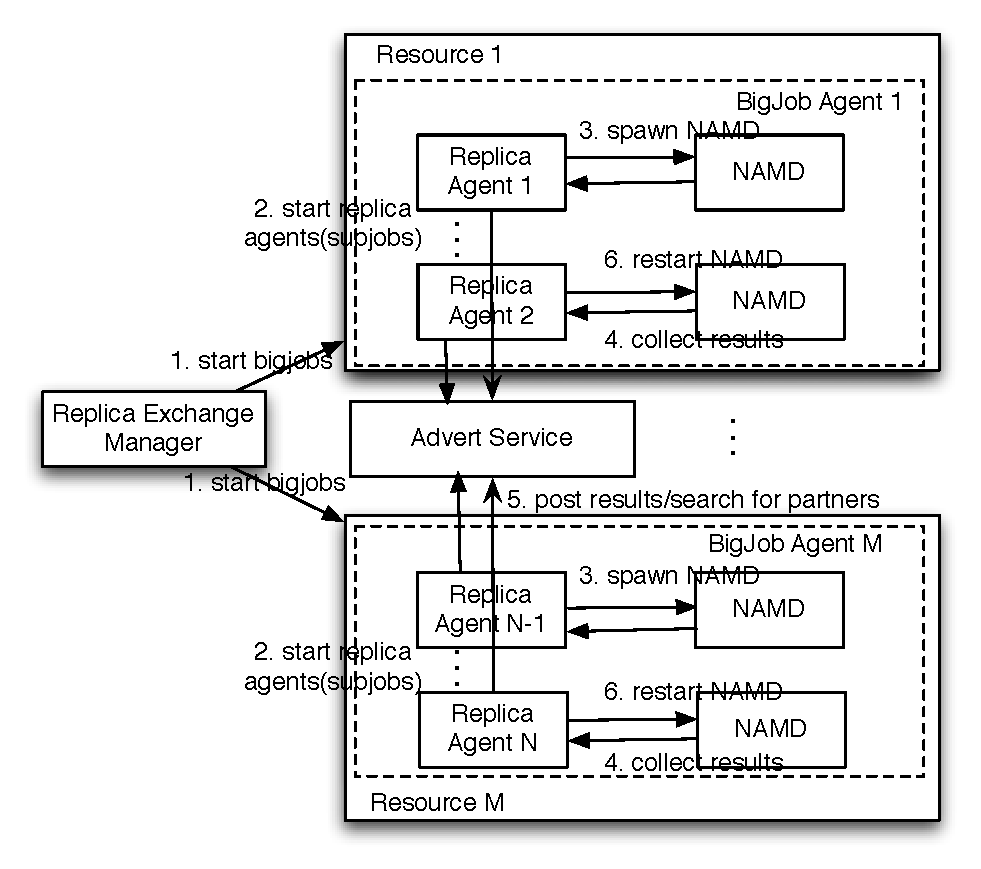
\includegraphics[width=0.9\textwidth]{asyncre.pdf}
% %\label{fig:async:b}
% \caption{\small Decentralized control flow: In the decentralized asynchronous RE, for  each replica there is a replica agent which individually manages the replica.}
% \label{fig:decent}
% %\vspace{-1em}
% \end{figure}

\alnote{we should write Case consistently with small or capital letter}
% We have to bear in mind that while Case II and Case III both implement the same asynchronous RE algorithm, they do it differently.
% At first glance it appears to be a question of philosophy, whether to
% let the replicas be managed by a master or to let each replica be
% managed individually.
%There could be implications effecting the performance of the
%algorithm. Where as in Case II, the master has to manage all the
%replicas and since it can only manage one replica at a time, although negligible, it is a cause for concern with large number of replicas. %The effect could be negligible and might now effect the overall performance.
%But the decentralized version (Case III) has no
%such issues as each replica is managed individually. % \jhanote{The distinction between Case 3 and 2 needs to
%  be made more clear. The following is ``implementation detail''. What
%  is the conceptual difference between Case 3 and Case 2?}

\section{Scale-Up and Scale-Out: Experiments and Results}

%
%%%%% FIGURE %%%%%
\begin{figure}
\centering
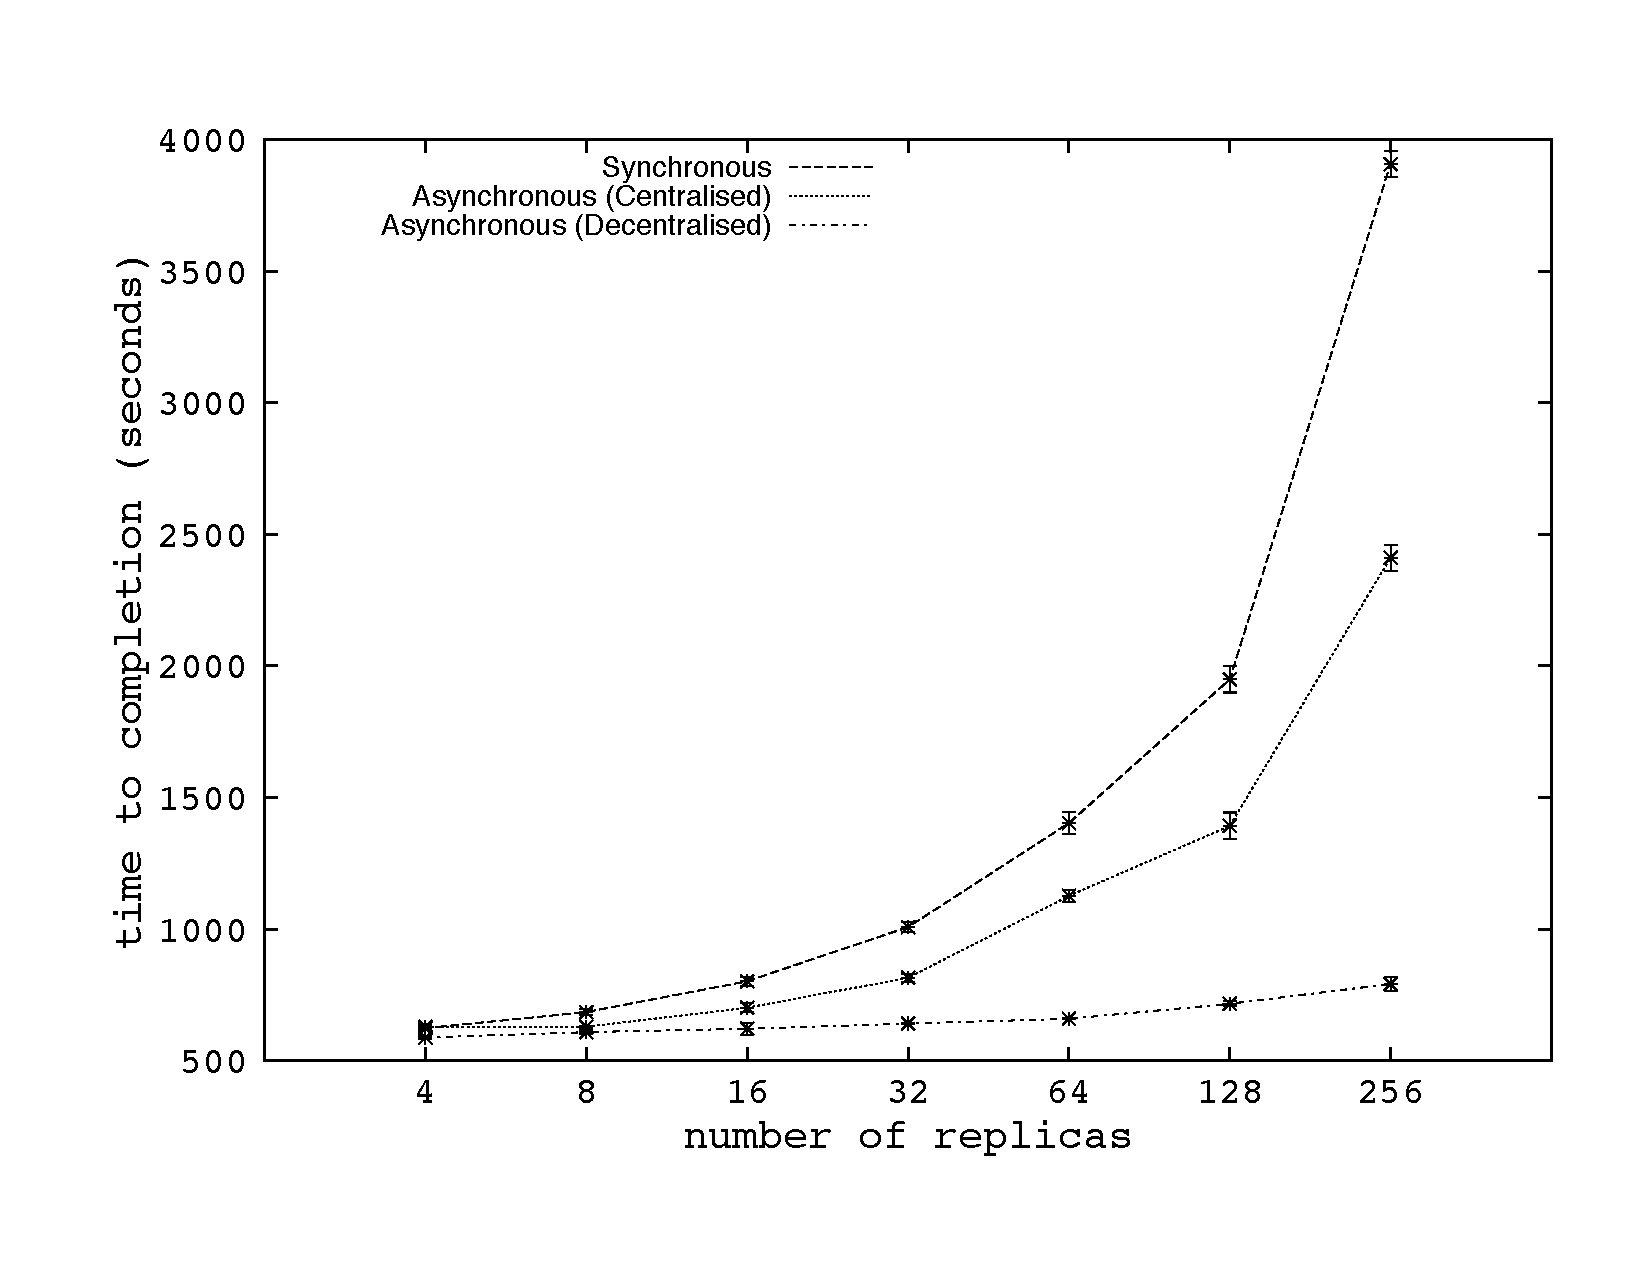
\includegraphics[width=0.9\textwidth]{../data/scale_up.pdf}
\caption{\small The graph shows the mean run times of synchronous and asynchronous - centralised/decentralised RE simulations on one machine. We repeated the experiments with up to 256 replicas. Up to 128 replicas, the experiments were conducted on QB and 256 replicas experiments were conducted on Ranger.}
\label{fig:graph}
\vspace{-1em}
\end{figure}

%While the traditional RE limits the exchanges to only neighboring temperatures, an asynchronous RE does not. This is not a concern when the number of replicas is small and there is little chance of an exchange between non-adjacent temperatures. However, as the number of replicas increases, the difference between the target temperatures becomes small enough to allow exchanges between non-adjacent temperatures. This also allows for 'crosswalks' to happen. The larger the number of crosswalks, the better is the performance of the simulation.

%To evaluate the performance of the various models of RE we have discussed in the abstract, we conducted several experiments on Teragrid and LONI resources. 
%In the following sentences we will analyze the performance of synchronous RE(Case I) with centralized asynchronous RE(Case II). 

\subsection{Scale-Up}

\subsubsection{Experiments}
In this section we describe the experiments we did increasing the number of replicas on a single machine. We configured the Cases I, II \& III to run parallel NAMD simulations with 4, 8, 16, 32, 64, 128 and 256 replicas sampling a temperature between 300 and 3000 K on Teragrid machines QueenBee and Ranger. \alnote{What resource?} In each simulation, one BigJob is launched with sufficient cores while each replica uses 16 MPI processes and runs 500 time steps between exchange attempts. Up to 128 replicas, all simulations were conducted on QueenBee, but the 256 replica simulations were conducted on Ranger as QueenBee allocates a maximum of 2048 cores per job. The metric used for comparison of 4, 8, 16, 32, 64, 128 and 256 replicas is the time to complete 16, 32, 64, 128, 256, 512 and 1024 attempted exchanges, respectively. It should be noted that the ratio between the number of replicas and the number of attempted exchanges is kept constant, for the purpose of comparison between each of these cases. It means that we are keeping the number of times each replica restarts, approximately, a constant. 

The mean run time is obtained by subtracting the queue wait time of the BigJob from the total time. As the ratio between the number of replicas and number of exchanges is kept constant, ideally, the runtime must remain constant too. In the graph (Figure~\ref{fig:graph}), we see an increase in the time to completion as the number of replicas increases. The increase in the completion time is not uniform across the three cases. We see the most slow down in case I and the least in case III.

\subsubsection{Scale up performance: Results and Analysis}

{\it Results:}\\

{\it Analysis: } From the graph (Figure~\ref{fig:graph}), we see that
Case I does not scale very well when we increase the number of
replicas. This is due to an inability to start and end all the
replicas at the same time and also due to the centralized control of the workflow. With more and more replicas, the time to start the replicas increases  and 
synchronization cost tends to increase too.  In Case II, the exchanges happen in
an asynchronous manner, but they are still conducted by the master
alone. As the number of replicas increases, the master quickly becomes
a bottleneck. But in Case III, the exchanges are all carried out in a
decentralised manner. Many exchanges can occur between different pairs
of replicas at the same time. Therefore, we say that the asynchronous
RE algorithm scales better and that the decentralised implementation
is better than the centralised implementation.

%
%%%%% FIGURE %%%%%
\begin{figure}%
\centering
\subfigure[Central]{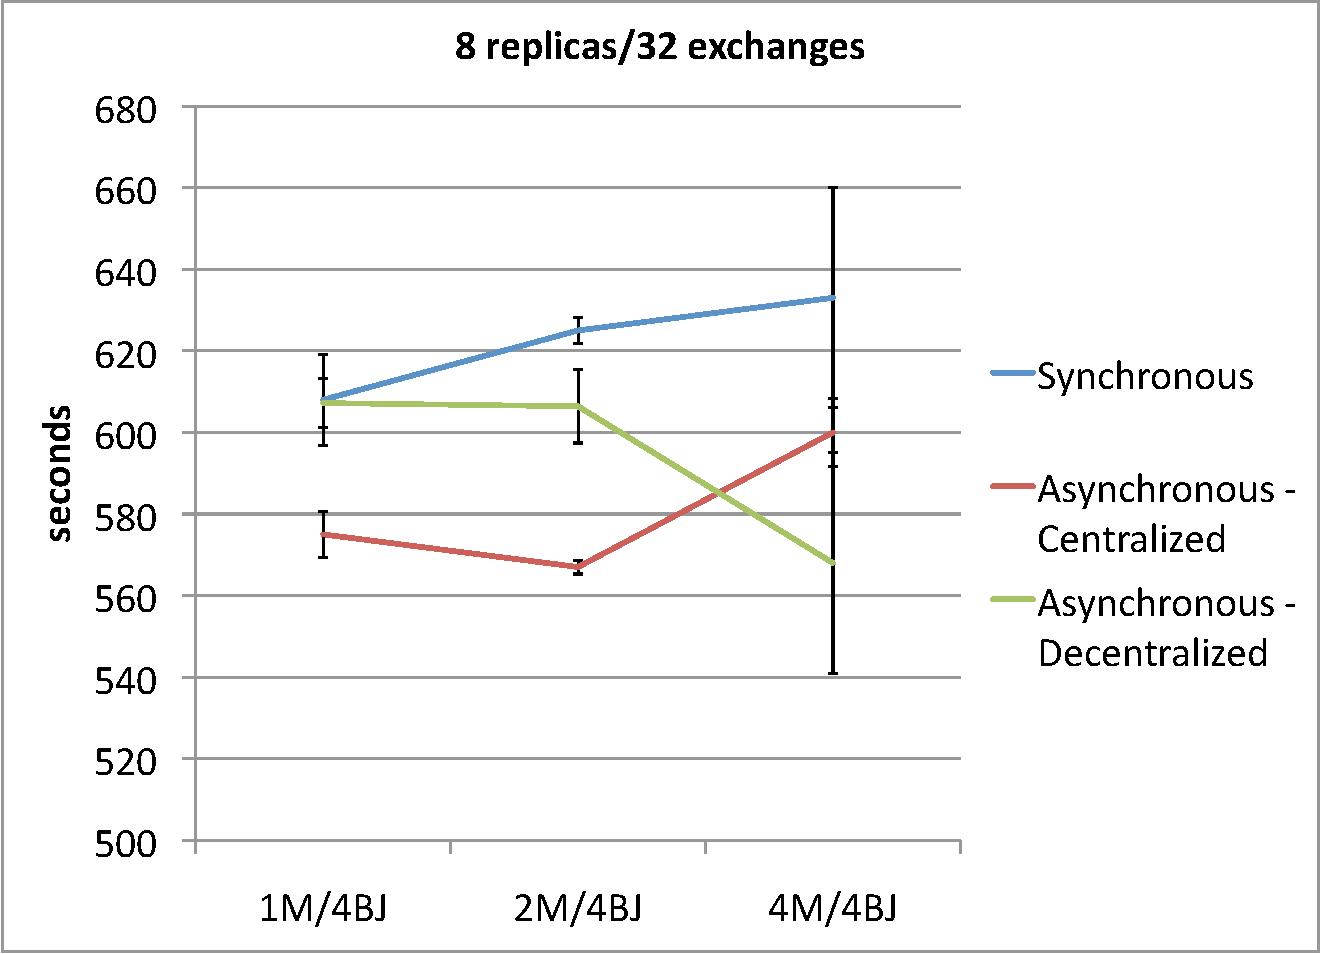
\includegraphics[width=0.47\textwidth]{../data/8rep.pdf}}\qquad
\subfigure[Decentral]{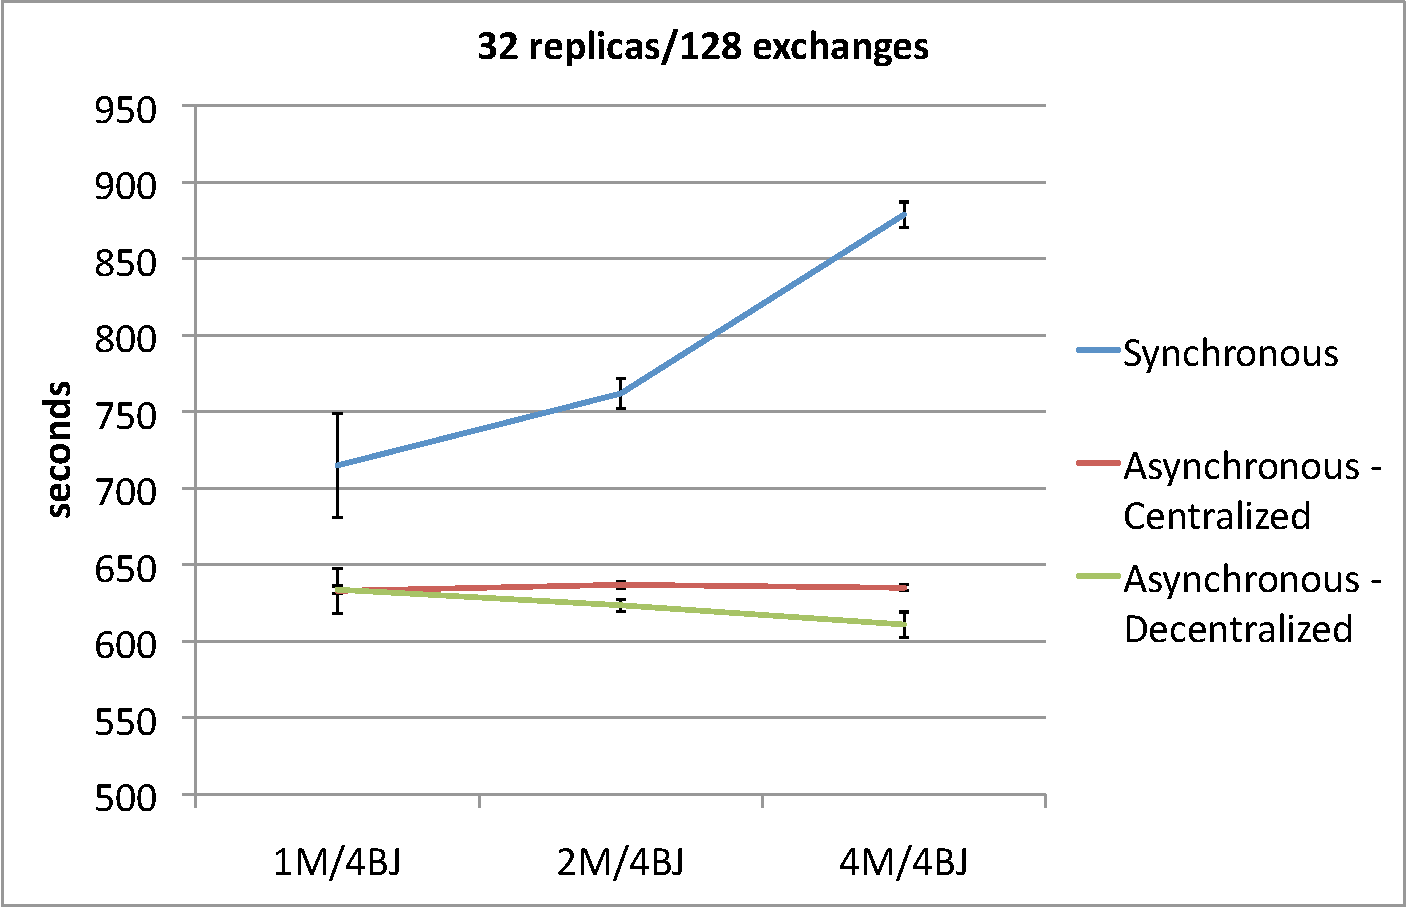
\includegraphics[width=0.47\textwidth]{../data/32rep.pdf}}\\
\caption{\textbf{8 and 16 replicas distributed:} The graph shows the mean run times of synchronous and
  asynchronous - centralised/decentralised RE simulations across two
  and four machines.}
\label{fig:24machines}
\end{figure}

\subsection{Scale out}

\subsubsection{Experiments}
In this section, we describe the experiments we did while increasing
the number of machines across which the experiments were done. We
chose LONI and Teragrid machines to run the experiments. We did
experiments distributed across two and four machines with 8, 16 and 32
replicas distributed equally across the machines.
Figure~\ref{fig:2machines} and Figure~\ref{fig:4machines} show the
behavior of Cases I, II and III across one, two and four machines,
respectively. Overall, there is not much difference between the local
and distributed runs in any case. The reason being that there is very
little interaction between the replicas. A very small configuration
file is staged to the remote machines after an exchange, which will
not add more than a couple of seconds per exchange. The rest of the
co-ordination is done via the advert service, which is usually located
on a remote machine in any case. Each query to the advert server is in
the order of milli seconds and does not produce a noticeable effect on
the performance.

\jhanote{There are several parts of the above paragraph that should be
  in the results sub-section. Similarly, there are parts in the
  experiments section for 'scale-up' that should be in the results
  section}

\subsubsection{Scale out performance: Results and Analysis}

{\it Results:}\\


{\it Analysis: } In Figure~\ref{fig:2machines}, we see the performance of all three cases when run in a distributed manner across two machines. As the data that is exchanged between replicas is very small, the Cases I, II and III behave in a similar manner to the way they behave on a single machine. \alnote{we should add some numbers and maybe a graph for an example scenario: x: machines y: time-to-solution} Again, asynchronous RE is better suited for distributed runs and the decentralised implementation scales best. The reason is, since each replica has its own replica agent, there is no need to transfer any files between machines. The required configuration files are created locally by the replica agent.


%In Case I, the pair-wise replica exchange can occur only between replicas of the same generation. Therefore, each exchange step is attempted only after all the replicas have finished running. After the exchange, all the replicas are restarted sequentially. This inserts a delay between the start time of the first replica, the last replica and the replicas in between. %As more resources become available at different times, the replicas already running or done are forced to wait for the newly running replicas to finish before moving on to the next exchange step. %Each exchange step is counted as an exchange.
%In Case II, the pair-wise replica exchange can take place between any two replicas in the ensemble irrespective of generation. As more resources become available, the new replicas join the ensemble immediately and the replicas already running are not restrained from attempting exchanges or restarting. This gives the asynchronous or synchronous RE a slight advantage. But with a large number of replicas we could easily see large difference.
%\athotanote{Further, we show performance gains by running across more than one machine. By running across more than one machine, we demonstrate the ability to divide the jobs into smaller sub-jobs and then distribute them across a number of machines, thereby reducing the risk of long queue wait times on an over-crowded resource. In Figure~\ref{fig:graph}, it can be seen that the asynchronous RE time to completion improves almost by a factor of 3 when moving from one machine to four machines. This was caused due to the fact that when the experiment was done on one machine, by the time the experiment ended, only 64 cores were allocated by the resource manager. But on the other hand, when the experiment was launched across four machines, it received an allocation of 64 cores on each of the four resources. The improvement that is seen in the case of synchronous RE from one to four machines is also due to a similar reason.} %The asynchronous RE appears faster by a couple of minutes due to the fact that when the BigJobs become available randomly, the synchronous RE has to wait for the newly running replicas to finish.

%slightly over 2 machines, but again increases over 4 machines. This is due to the fact that the experiments have been run only a handful of times but, over time, it can be assumed that it will result in reduced queue wait times.

\section{Conclusion}



%\athotanote{is this right? }
% We are also going to have a wider group of replicas to look at for
% each replica as we are not pairing the replicas.

% Also, we have the usual advantages of using a pilot-job,
% such as reduced queue wait times by not having to submit to the queue
% at every step.  We also provide major advantages when compared to
% Parashar et al.

%  to run the asynchronous RE simulations,
% including the ability to run MPI
% jobs.
% ??We need to evaluate the performance of our models and compare with other models for conducting replica exchange simulations.


%%%%% FIGURE %%%%%
%\begin{figure}
%\centering
%\subfigure[Time to complete 64 exchanges on QB with two 64 core BigJobs and on both QB/Louie jointly with a 64 core BigJob on each machine.]{
%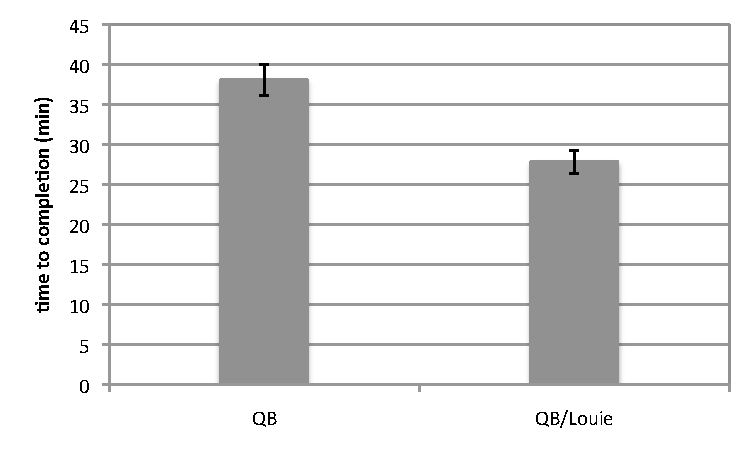
\includegraphics[width=0.40\textwidth]{figures/graph1.pdf}
%\label{fig:subfig3}
%}
%\hspace{0.5cm}
%\subfigure[Time to complete different number of exchanges on QB/Louie with a 64 core BigJob on each machine.]{
%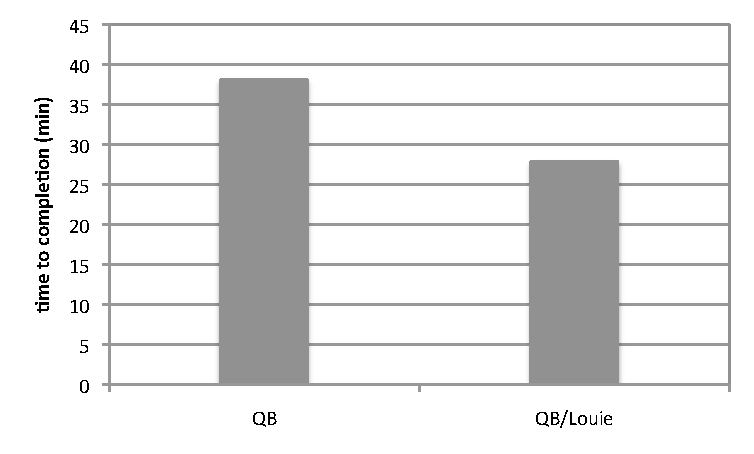
\includegraphics[width=0.40\textwidth]{figures/graph2.pdf}
%\label{fig:subfig4}
%}
%\caption{\small In Figure 2(a), we can see the improvement in performance when run on more than one machine. It is due to the fact that usually the first queued job becomes active before the second on a machine and running jobs on more than one machine solves this problem. In Figure 2(b), we can see consistent performance over prolonged runs, making 32, 64 and 128 exchanges.}
%\label{fig:graphs}
%\vspace{-1em}
%\end{figure}
%%%%% FIGURE %%%%%

An important motivation for this work is to implement a scheme that does not depend on a
static, well defined model of resource availability. %We test and scale
%our implementation on production level grids such as Teragrid and
%LONI~\citep{LONI_web}.
Preliminary results, shown in Figure~\ref{fig:graph}, indicate the
most important advantages of asynchronous RE and SAGA/BigJob over
traditional RE: (a) allows for exchanges to occur between replicas
with non-nearest temperatures, which in turn allows crosswalks to
happen (b) a reduced time to completion when running on more than one
machine due to improved resource availabilities, (c) the advantage of
using a pilot-job mechanism, which eliminates the waiting times at the
local resource manager, \alnote{have shown this in prev. papers, but
  we don't really have data in this one} and (d) the ability to scale
out across different production level infrastructure, such as, the
Teragrid and LONI.
% It performs well even after doubling and quadrupling the number of
% exchanges required to complete the simulation. The time to
% completion only increases by 35\% after doubling and 117\% after
% quadrupling the number of exchanges.
%\athotanote{should the results
%  be included in the conclusion or in a separate results section? Do
%  you agree with the \# of exchanges scheme to show the data?}
% Unfortunately we have results only for Case II currently, but 

%In summary, we have established the ability to scale-out across different
%infrastructure and compared the performance of the asynchronous
%RE with the synchronous RE at large scales. 
Further, we compare the traditional RE model (case I) and the centralised (case II) and decentralised (case III) models of the asynchronous replica exchange by modeling and repeating the experiments a reasonable number of times, so as to accurately quantify the scientific and performance gains. %We also propose to measure the frequency with which crosswalks occur with increasing number of replicas and measure the advantages due to a decentralized implementation in the full paper.


%With this asynchronous replica exchange mechanism we can improve the
%number of exchanges per unit time, a key parameter in judging the
%performance of a replica-exchange mechanism. \athotanote{is this
 % right? }  We are also going to have a wider group of replicas to
%look at for each replica as we are not pairing the replicas. Also, we
%have the usual advantages of using a pilot-job, such as reduced queue
%wait times by not having to submit to the queue.  Unfortunately we
%dont have results \jhanote{What results can we present -- any? some?},
%so we will say, (i) we establish the ability to scale-out (distributed
%and exa-scale) across different infrastructure (ii) compare the Async
%versus sync formulation at unprecedented scales \jhanote{At least
%  outline what infrastructure we / you are planning to use?} (iii)
%compare different implementations of the Async version
 

\begin{acknowledgement}
  This work is part of the Cybertools (http://cybertools .loni.org)
  project and primarily funded by NSF/LEQSF (2007-10)-CyberRII-01.
  Important funding for SAGA has been provided by the UK EPSRC grant
  number GR/D0766171/1 (via OMII-UK) and HPCOPS NSF-OCI 0710874. This
  work has also been made possible thanks to computer resources
  provided by TeraGrid TRAC TG-MCB090174 and LONI resources.
\end{acknowledgement}

\bibliographystyle{kluwer}
\bibliography{saga,literature}    
\end{document}

